% TODO: Mention here about the 8% assumption
% http://www.thornburginvestments.com/pdfs/TH1401.pdf
% http://www.investopedia.com/articles/investing/052913/inflations-impact-stock-returns.asp

\chapter{Stashing Your Cash}
As you earn more and spend less, your money will start accumulating. You will need to put it somewhere. This is the third piece of financial independence: investing. How you invest your money is very important because it will eventually become your source of partial or entire income. As your savings accumulate, it will become increasingly important to have a sound investment strategy. It may not seem quite so important at the beginning, but the magic element of investment growth is time, so the choices you make early on will be magnified over time.

The best investment strategies require very little maintenance. People who invest in something solid and leave it there tend to do better than those who move their money around a lot. So, once you find an investment strategy you feel comfortable with, you'll essentially be done. The rest is just investing according to that strategy. Do this early, and then you can focus on the rest.

The basics of investing are fairly straightforward and can be used by most people to develop a fairly decent set of investments. Like many subjects, it does have a lot of depth, but it's up to you how deep you'd like to tread. The deeper you go, the more efficient and effective your investments will be, so it's worth the effort. This book is based on the assumption that you are willing to do a lot of your own research and put a lot of effort into finding the most effective way for you to earn, save, and invest your money. Therefore, I go into some depth in this book, but this is still just scratching the surface. There are some books I highly recommend for you to complete your investment training. Nonetheless, even in this book, I try to make it easy for you to choose for yourself how deep you want to go. I will present some easy and increasingly complex investment strategies, and let you decide.

\section{Disclaimers}
Investing isn't brain surgery, but it does share one thing with it: practiced incorrectly, it can be disastrous to your health (your financial health). While what I present here is time-tested and recommended by many of the top investors and academic economists in the country, I am not a certified financial planner. I'm just someone who has studied this extensively and has been able to use this knowledge to retire at an early age.

If you choose to do your own investing, which I recommend, you're taking the risk of misunderstanding something you read, not noticing or not taking warnings seriously when you read them, or otherwise incorrectly executing what you learn. On the other hand, if you don't do your own investing, you're taking the risk that your financial planner is either incompetent, doesn't have your best interests at heart, or both. Unlike brain surgeons, who risk malpractice lawsuits, financial planners are more likely to take advantage of their clients, and the legal regulation of the financial planning industry is nothing compared to brain surgeons. It's up to you to decide whether it's worth the risk to trust a financial planner.

There are several other risks you face by investing, and it's impossible to eliminate them all. Even if you invest in only government bonds, assumed to be the safest investment around, you face \emph{inflation risk,} which is the risk that the money you've invested will be able to buy less in the future, and \emph{interest rate risk,} which is the risk that the interest rates will change. Most intelligent investors believe the inflation risk of government bonds alone outweighs any of the other risks. These include, but are not limited to, \emph{currency risk,} which is the risk that the value of the currency your investments are held in will change by switching to a different currency; \emph{liquidity risk,} which is the risk that you won't be able to “cash out”; \emph{financial risk,} which is the risk that companies or governments will face some internal disruption; \emph{market risk,} which is the risk that supply and demand will significantly affect your investments; and \emph{credit risk,} which is the risk that loans won't be paid off.

In other words, it's possible you're going to ``lose your shirt,'' ``take a bath,'' or whichever cliché you prefer for ``lose way more money than you ever dreamed possible.'' This can be scary for some people, and thrilling for others. It might keep you up at night. It might give you chills. The risks are there, and you should know about them, so you can invest with your eyes open. The whole point of this book is awareness of trade-offs, and risk is one of the factors you must consider when you weigh your trade-offs. One of the cardinal rules of investing is the trade-off between risk and return. When one goes up, the other always goes down.

There are many ways to manage risk, which I will discuss at length. If you know your risk tolerance when you go in and invest accordingly, it shouldn't be too scary. It only gets scary when you get in way over your head, taking on more risk than you can handle. For this reason, if you're not experienced with investing, I recommend that you start out conservatively, assuming you have a higher risk tolerance than you may think. After some experience, you can adjust it. Nonetheless, you may decide that those risks are worth the reward. That's your choice.

Despite all the risks, it's still better to invest than not. It's impossible to avoid investment risks, even if you avoid investing entirely. You still have \emph{job risk,} which is the risk that the company you work for invests poorly and lays you off; \emph{economic risk,} which is the risk that the economy as a whole plunges, leaving you out of work entirely; and the biggest risk of all: \emph{opportunity risk,} which is the risk that you will miss out on investment opportunities. A lot more money is lost from opportunity risk than all the other risks combined.

\section{Investing basics}
Like spending, investing is also very personal. Your investment strategy will depend on a number of factors specific to you. One is your \emph{age} and \emph{time horizon.} The younger you are or the further out your goal is, the longer you have to weather volatility in your investments. If you can weather short-term risk then you can gain higher long-term returns. Another is your goal. In the case of this book, I will assume your goal is financial independence. Another is your \emph{risk tolerance,} which is a measure of how emotional you get when your investments go up and down. All three factors should be measured and accounted for in your investment strategy.

There are many different \emph{investment vehicles,} or places to put your money, that will give you some interest or return. The most important investment vehicles are stocks and bonds.

A \emph{stock} is a small piece of ownership of a company or asset, like real estate or precious metals. You literally own part of the company, or a share of assets, and you get paid a chunk of its earnings, which are called \emph{dividends.} You may also sell stocks on the open market, and how much you can buy or sell it for can vary drastically over time. Any gain you get from selling a stock for more than you bought it is called a \emph{capital gain.} Stocks are the most powerful investment vehicle around for long term investing, because they provide the greatest long term return, although they also involve quite a bit of short-term risk.

A \emph{bond} is a share of a loan. Organizations, usually governments or businesses, need loans for temporary needs, much like a homeowner would take out a loan for an improvement on their house.  However, these institutions need much larger loans than homeowners, so they divide it up into many smaller loans, called bonds. These bonds have an interest rate, sometimes called the \emph{coupon,} which is a certain percentage of the bond that the bond seller promises to pay you in addition to paying back the loan. Like stocks, you can buy and sell bonds on the open market, so in addition to the interest, you can also get a capital gain from bonds. There are also \emph{zero-coupon bonds,} which don't pay interest but are sold at a \emph{discount} from their \emph{face value,} which it will be worth on its \emph{maturity date.} Basically, you buy these bonds for a certain price, and on a specific date, the organization promises to pay you back a higher amount.

A \emph{mutual fund,} or just \emph{fund,} is an aggregation of many stocks, many bonds, or both together. This is the most common way to invest, because it's the easiest and cheapest way to diversify, which I will explain shortly.

Here are some other investment vehicles you should know about:
\begin{itemize}
\item \textbf{Savings account} -- An account at a bank that pays interest, which often has limitations on how often or how easily you can withdraw money. The ease with which you can withdraw money is called \emph{liquidity.} Savings accounts are very liquid, but not as liquid as checking accounts.

\item \textbf{Money market fund} -- This is like a savings account, but it offers limited check writing capabilities, and it used to offer better rates than savings accounts, but now they offer roughly the same rates. Traditionally, money market funds weren't covered by \emph{FDIC insurance,} a government guarantee in case the bank goes under, so they had more risk than savings accounts, but that has changed in 2008. Nowadays, you can pretty much treat money market funds like savings accounts that sometimes offer a limited check writing feature.

\item \textbf{CD, or Certificate of Deposit} -- This has a date (called the \emph{maturity date}) that you must wait until before you can withdraw money. This can be anywhere from one month to several years. Having to wait to withdraw obviously means it's not as liquid as a savings account, and in exchange for promising to wait, you're supposed to be rewarded with a higher rate of return. I usually find this reward to be small or non-existent compared to money market funds, so I don't bother with CDs.
\end{itemize}

\section{Schools of thought}
There are many different schools of thought and points of debate in investing, particularly in stocks. One debate is over \emph{long-term investing} versus \emph{day trading.} Long-term investors believe that the best strategy is to buy good investments and keep them as long as possible, while day traders time their investments so they can buy low and sell high. The traders themselves debate between \emph{fundamental analysis} and \emph{technical analysis.} Fundamental analysis focuses on the fundamental aspects of a company, such as how much money they have and how much they earn. Technical analysts simply look at past trends of stock prices and try project those trends into the future.

Another point of debate is over \emph{value investing} versus \emph{growth investing.} Value investors look for good companies that are going through tough times, so they can buy them at low prices, kind of like looking for sales at your supermarket. Growth investors look for good companies that are very successful and seem poised for future growth, irrespective of their cost. Many investors employ some combination of both strategies.

Another debate among long-term investors is the importance of \emph{diversification.} Also called \emph{asset allocation,} diversification means owning several different kinds of investment vehicles, and stocks in particular, that tend to behave in different ways. It's argued that this will provide a greater return with less volatility and less risk. Others believe that owning so many stocks means owning a lot of dead stocks, which dilutes the returns. They argue that you need no more than 15 different stocks to sufficiently manage risk, so if you can pick 15 really good companies, you'll do better than if you have hundreds or thousands. Many asset allocators argue that it's impossible to predict which companies will be successful, and that most people tend to get better returns by aiming for the average than by trying to pick the right stocks. This is called the \emph{random walk theory.}

A more recent debate is over \emph{socially responsible investing, or SRI.} This is investing with your conscience, only owning companies that have a record of treating employees, communities, and the environment ethically. SRI investors argue that, in addition to being better ethical choices, these companies also perform better over the long run because they have happier customers, happier employees, and fewer lawsuits. This is a relatively new twist in investing, so it's hard to tell how well it actually works in practice, over the long run. The biggest known disadvantage of SRI funds is that they tend to cost a lot more than non-SRI funds. Maybe the only real advantage of SRI funds is that investors feel better about the ethical aspect of their investments. This may be intangible, but it is nonetheless important.

I've toyed with every approach to investing and trading I've talked about. They each have their pros and cons. You'll hear a lot about all of them if you pay attention to the investing media. But I needed to converge on a strategy for my own needs, and for that, I decided to mostly ignore the media, which seemed to be all over the board. The media, I realized, has no incentive to measure and quantify the effectiveness of each of these strategies, and report on that. The media's goal is to have a lot of readers and viewers. That's all. For that, they need excitement, and what is more exciting than a lively debate? They also emphasize day trading over long-term investing because day trading is a lot more exciting. Long-term investing is about as exciting as watching plants grow.

I decided to focus my attention on the experts, those who aren't trying to stir up debate, entertain audiences, or sell their own products, but are only trying to find which strategies have proven to be the best. These are the academic economists and the most successful private investors. The most successful investor, of course, is Warren Buffett. The economists that seemed the most trustworthy to me were Burton Malkiel and John C. Bogle. When I focused on these experts, I found very little debate. They were mostly in agreement, and recommended the same strategy for average investors, based on \emph{Modern Portfolio Theory,} which I will explain later in this chapter.

\section{The problem with bonds}
\emph{Your Money or Your Life} recommends owning only one investment vehicle: bonds, issued by only one entity: the U.S. Government. This does have certain advantages. It has the least volatility and least risk of losing money. Its low volatility means that you don't need to mess around with withdrawal rates (which I mentioned briefly in the last chapter, and will talk more about in Chapter 5) because you can count on being able to spend exactly what the bonds pay.

However, this strategy has one fatal flaw: \emph{inflation risk.} Because these bonds are so safe, they also have very low return. Often, its rate is less than inflation, which means that you'll not only not earn enough to pay for your retirement, but you'll be losing money. \emph{Your Money or Your Life} makes some arguments for why inflation is irrelevant, and it may be true that inflation is less relevant for people who are frugal. There is some debate as to how to measure inflation, and how effective those measurements actually are. However, inflation is still a very real risk. There is also opportunity risk, which means that the inferior growth of government bonds will cause you to unnecessarily delay your financial independence.

There is only one investment vehicle that is practically guaranteed to out-pace inflation: stocks. The reason is that inflationary price increases are made by companies, which means more income, which means more dividends and capital gains for investors. Most companies grow in many ways other than inflating prices, so they are able in out-pace inflation. You must out-pace inflation if you expect to live on your investments. For the sake of diversification, you should have some bonds in addition to stocks, but the majority of your investments should probably be in stocks.

Yes, you can lose a lot of money with stocks. They can be risky if not used properly, but the risk can be managed, which I will explain later. The most important thing about stocks and corporate bonds is that most of the risk is short-term. One year, they may drop significantly, maybe even for years at a time, but they always go back up eventually, short of a severe economic meltdown or collapse of the United States government, in which case, you've got bigger problems than the value of your investments. Even if you bought all your stocks right before the stock market crash in 1929, you still wouldn't have lost money if you'd held them for at least 10 years.

There is a new form of U.S. Treasury Bond that is specifically designed to beat inflation. It's called \emph{TIPS,} which stands for \emph{Treasury Inflation-Protected Securities.} They take last year's inflation rate, measured by a standard index, and then pay some rate on top of that. This is a tool for managing inflation risk in Treasury bonds. If you really want to invest in only Treasury bonds and live on the interest, as suggested in \emph{Your Money or Your Life,} I'd recommend using TIPS. However, this still doesn't manage the \emph{opportunity risk} or \emph{interest rate risk.}

Since there are ways to manage the risks of investing in stocks and corporate bonds, I believe these are the best investments for financial independence. I recommend you use these, but it's your money, so invest it in whatever what seems best for you. I will be discussing stocks and bonds for the remainder of this chapter.

\section{Investing made easy}
Learning about investing often makes people's eyes glaze over. In this chapter I briefly explained all the absolute basics of investing, without much detail. If you want more detail, you should do more research. Check the Resources section at the end the book. What I'm going to do here is explain the strategy I recommend for financial independence, how that strategy works, and why. That will involve a certain amount of detail, and although I will try to keep it as easy as possible, learning the details about investing necessarily means lots of numbers, \% and \$ signs, and new jargon that I will be introducing along the way.

I don't want you to feel overwhelmed by this and tune out, or worry that this is over your head and maybe this financial independence stuff isn't for you after all. As I said at the beginning, this path will require time and effort, learning new things, and doing some research. It's important to learn the details, and that's why I'll go over it. But it's not essential for achieving financial independence. Without an in-depth knowledge of investing, it may take you longer to achieve, since your investments won't be as efficient, but it's still possible. If you choose this path, then here are three easy investment choices.

One approach, of course, is to \textbf{hire a financial planner,} essentially out-sourcing your investing. They'll interview you, ask you basic questions about your financial situation and goals, and come up with a plan that works for you. They will describe it in simple terms, and if you feel comfortable with it, you'll write them a check, and you're good to go. They'll continue to work with you, so if you ever have questions or concerns about your investments as the economic weather changes, you can call them up. They'll keep you from doing deadly things like buying into the latest fad or selling everything when you get scared.

However, planners are \emph{very} expensive, and these costs come straight out of your investment growth. Few investors fully appreciate just how much these costs hurt their investments over time, and many planners are loathe make this too clear. They argue that their returns are so fabulous that your costs will be covered many times over, but research into this industry does not bear this out. Most financial planners match the returns of the market as a whole, and many even under-perform the market, so the costs matter a great deal.

To make matters worse, incompetence is rampant in this field. Most planners are trained more in sales than in investing, and their certification process isn't very impressive. Make sure you get a referral from a trusted source, and interview the planner thoroughly. Ask to see how their other portfolios have done, ask how their fee structure works, and shop around. To fully appreciate the impact their costs will have, ask for a comparison between how much money you could reasonably expect to have in several decades without costs versus with their costs. Make sure they understand and support your financial independence goals. Some will tell you it's not possible, but usually that just means they don't know how.

Hiring a financial planner is theoretically easy, but the minefield of high costs and bad planners definitely sours it. Recently, Vanguard started offering full-service financial planning. Vanguard is by far the most trustworthy investment company in the industry. They consistently offer the lowest fees and the best customer service. Vanguard is owned by their fund shareholders, which better aligns them with their interests. If you decide to hire a financial planner, I urge you to go with Vanguard. I have no personal financial stake in this, only a philosophical one. See the Resources section for the website.

Vanguard also offers a \textbf{one-time financial planning service.} This isn't a full-service option. The less management you're paying for, the more money you get to keep in your investments. They'll interview you, develop a customized asset allocation plan, and explain how to manage it yourself, which is really easy. The cost depends on your initial investment. It's a flat fee, so although it feels like more up-front, it's actually much cheaper than any financial planner because it's only a one-time fee, rather than consuming a percentage of your investments every year. See the Resources section for the website.

Another easy approach is to \textbf{buy a pre-packaged portfolio} called a \emph{balanced fund,} which is as easy as opening a savings account. You buy one fund and that's it. They take care of the allocations. All you'd need to do is call up the fund provider and ask for the fund, and then send them your deposits. Balanced funds are easy and cheap, but they are fairly generic, not customized to your needs, so they may not provide the optimal performance and risk management for your needs. If you'd like to go with balanced funds, again I would recommend Vanguard's All-in-one funds. They have a really easy online system that asks about your goals, your age, and your tolerance for risk, and then recommends a fund. See the Resources section for the website.

If you'd rather take total control over your own investments, and you're ready to venture into the wild and exciting world of investing, read on!

\section{Modern Portfolio Theory}
The investing strategy I recommend is buying and holding a well-diversified portfolio of low cost index funds of stocks and bonds, employing Modern Portfolio Theory.

\emph{Index funds} are mutual funds that just buy and hold shares that track a market index, which represents some segment of the stock or bond markets. The index rarely changes, so the fund also rarely changes. The index represents the average return of these markets, but since taxes and fees are much lower, you can expect above-average returns from them. Index funds may sound mediocre or even drab, but they're actually very powerful in their simplicity. Despite their enormous fees, most mutual funds usually \emph{under-perform} the indexes, often with \emph{more risk.} When you add the huge overhead of fees and taxes, index funds almost always out-peform most funds. It is possible to find that rare fund that can out-perform index funds, but it's impossible to know ahead of time which funds those will be. Most of yesterday's stars are tomorrow's dogs.

\emph{Modern Portfolio Theory (or MPT)} is a Nobel Prize-winning investment theory which seeks to maximize investment returns while minimizing risk. It may seem almost magical when you first see it in action, but it's very real, and very powerful. In some ways, it has revolutionized investing, and put many of the debates to rest. A good way to describe MPT is ``the whole is greater than the sum of its parts.'' A good analogy is sodium chloride. Separately, sodium and chloride are explosive chemicals, but put them together and you get table salt. It sounds magical, but it's really quite natural. That's kind of how MPT works.

Modern Portfolio Theory is based on diversification, and \emph{asset allocation.} To diversify, you need to buy several different investment vehicles of many different types. Each investment vehicle is known to behave differently over time. By ``behave'' I mean how its prices tend to move on the open market. One investment vehicle might tend to zig zag wildly in its prices. Another one may tend to have a smooth trend upwards. Another might zig zag a little, but it's known that it doesn't tend to move quite in sync with the other two.

You get lots of these different kinds of investment vehicles, or \emph{asset classes,} together in a \emph{portfolio,} which is just a conceptual grouping of all your investments. So, for example, if you have \$10,000 to invest, you might put \$2,000 in bonds, \$2,000 in growth stocks, \$3,000 in value stocks, and \$5,000 in international stocks. That's a diversified portfolio of investments. Its asset allocation is 20\% in bonds, 20\% in growth stocks, 30\% in value stocks, and 50\% in international stocks. In each of these categories, you'd tend to own one or more funds, each of which may have hundreds or even thousands of individual stocks or bonds. What you end up with is a collection of funds, called a \emph{portfolio.}

Investors in the past didn't think much about their portfolio as a whole. It was just a collection of individual investments, and they focused on how each of these performed separately. MPT showed that the behavior of each of the parts plays off of each other to have different effects on the portfolio as a whole. The portfolio, if arranged properly, can have a higher return and lower volatility than any of the funds contained therein. I'll give an example of how this works. I'll use two fictitious funds that are extremely volatile and out-of-sync with each other. In real life, you'd never find funds like these, so returns like this are impossible. The point is to illustrate the concept, and an ideal case helps accomplish that.

Suppose you decide to invest \$10,000 in one of two funds that are known to be volatile, but give excellent returns over time (it's generally understood that the more volatile a fund, the higher its return over time).

You buy \textbf{Fund A} for \$10 per share. The next year it's worth \$5 per share, the next year it's \$2 per share, and the next year it's \$20 per share. Insane, scary volatility. It's doubled in price over three years, but it was on quite the joy ride along the way. Had you invested in only this fund, then after three years, your \$10,000 would now be \$20,000. That would feel pretty good, but you weren't feeling so hot last year when your \$10,000 had shrunk to \$2,000!

Suppose instead that you chose \textbf{Fund B}, and you bought this fund for \$10 per share. Next year it's worth \$20, the year after it's \$25, and the year after that it's \$15. Had you invested in only this fund, then after three years, your \$10,000 would now be \$15,000. Still very good, but you're probably kicking yourself for not selling it last year when it was worth \$25,000!

Now let's suppose you used MPT and allocated your money 50/50 between both funds. Instead of \$10,000 in one fund, you invest \$5,000 in each of two funds. At some point, you employ a technique called \emph{rebalancing,} which means buying and selling whichever funds necessary in order to bring your allocation back to half and half. Let's see how you would have done.

You buy 500 shares of Fund A at \$10 per share, and 500 shares of Fund B at \$10 per share, which is \$5,000 in each, for a total of \$10,000. After the first year, your portfolio would be worth \$12,500. In the second year, it would be worth \$13,500. Notice how nice and smooth your growth has become? No more sleepless nights as you watch most of your money vanish in thin air, only to earn it all back and then some the next year.

At this point, you see that your allocation is way out of whack. You now have 7.4\% in Fund A and 92.6\% in Fund B, so you rebalance. You sell \$5,750 of Fund B, which is now priced very high, and use that money to buy more shares in Fund A, which is at a bargain price. Notice how rebalancing has a built-in effect of buying low and selling high, as you sold the high fund to buy more of the low fund. You now have only 270 shares of Fund B but 3,375 shares of Fund A, and you're back to half and half. Since it's so dirt cheep, you were able to afford a ton of shares. Next year, Fund B shoots through the roof at \$20 per share. Fund B ends at \$15 per share. You end up walking away with a portfolio worth \$71,550! That's much better than either fund separately, with much less volatility along the way.

\begin{figure}[htbp]
  \centering
  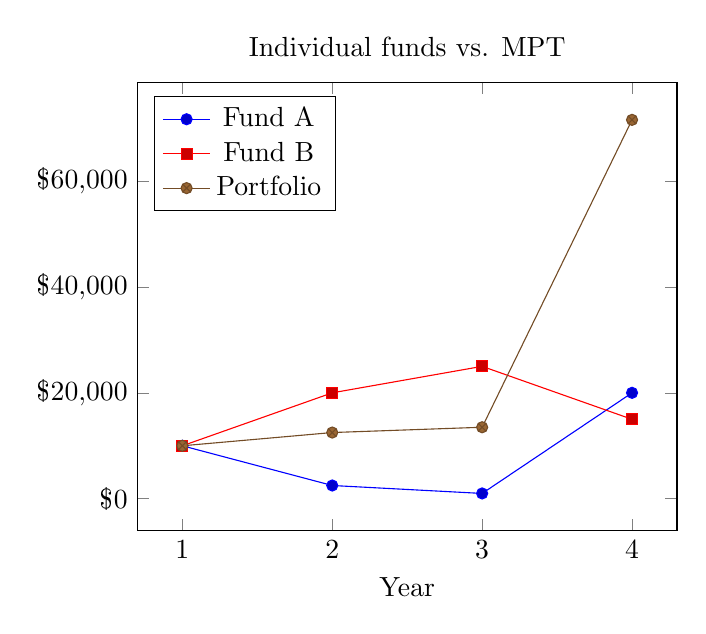
\begin{tikzpicture}
    \begin{axis}[
      xtick=data,
      scaled ticks=false,
      xlabel=Year,
      legend pos=north west,
      title=Individual funds vs. MPT,
      yticklabel={\$$\pgfmathprintnumber{\tick}$},
    ]
    \addplot coordinates {
      (1, 10000)
      (2, 2500)
      (3, 1000)
      (4, 20000)
    };
    \addplot coordinates {
      (1, 10000)
      (2, 20000)
      (3, 25000)
      (4, 15000)
    };
    \addplot coordinates {
      (1, 10000)
      (2, 12500)
      (3, 13500)
      (4, 71550)
    };
    \legend{Fund A, Fund B, Portfolio}
    \end{axis}
  \end{tikzpicture}
\end{figure}

Using MPT, you're able to combine funds in a way that is most likely to give this magical effect of higher returns and lower volatility. It depends on certain characteristics of each of the components, which the above example had in an extreme way.

The most important characteristic is that the funds must have as low a \emph{correlation} as possible. Correlation is a measure of how the funds tend to behave relative to the others. The funds I gave above always moved in exact opposite ways. When one went up, the other went down, and vice versa. This is called \emph{negative correlation,} which is the best possible situation you could have, and unfortunately almost entirely unheard of. It's like the holy grail of Modern Portfolio Theory. It's also extremely rare to get zero correlation, which is where the two components sometimes move in sync, sometimes not, and sometimes opposite, seemingly at random. The best you can hope for is a low \emph{positive correlation} where they will usually move in sync, but not perfectly in sync, with a little bit of zig zag away from each other here and there.

Another useful characteristic is for all of the components of your portfolio to perform extremely well over time. This is possible, but not if you want low correlation as well, which is the most important thing. The example I gave didn't just perform extremely well; they performed obscenely well. Obviously performance like that together with nearly perfect negative correlation is impossible, but the effect is the same, so it was good for illustration purposes.

In real life, the only two asset classes that have anything but nearly perfect positive correlation are stocks and bonds. Therefore, the only way to take advantage of the effects described above is to have some combination of stocks and bonds. Unfortunately, bonds don't perform nearly as well as stocks; often their performance is half of what stocks are. This definitely dilutes your returns, but it's the only way to keep volatility down. I will describe later why low volatility is so important for financial independence.
Another problem in real life is that you can't really predict the correlations. The correlations are volatile too. You can only go on probabilities based on past behaviors. Sometimes everything will move completely in sync, as it did in the October 2008 crash, which was quite brutal for everyone, no matter how diversified they were. Nothing was safe except Government bonds, and even those rates soon dropped to 0\%.

Finally, there's some question as to when is the right time to rebalance. You may have noticed in my example that I picked the perfect time to rebalance, right when both funds were at their extremes. How can you know when that time has come? You can't. You can only guess. One common technique, which is simple and works fairly well, is to rebalance every year, no matter what, but some research shows that two years or more works better. As long as you do rebalance occasionally and no more frequently than once a year, you should be fine.

You can also rebalance more strategically. One technique is to rebalance after a huge, sudden drop or spike in prices. These are the times that you will most gain the most advantage from rebalancing. Of course, such radical changes in the market tend to happen close to each other. You may rebalance after a big drop, only to see it drop significantly more a week later. If you're not careful, this can pull you into becoming a day trader, reacting to the daily whims of the market volatility, rather than the proven strategy of buying and holding.

I designed a more sophisticated approach to rebalancing. This approach only works for ETFs, which I'll explain later. The idea is to rebalance a fund only at the ideal times for that specific fund. Every month, I check the cash portion of my portfolio. If the percentage of cash in my portfolio exceeds my target allocation, I go into buying mode. If it's less than my target allocation, I go into selling mode. In buying mode, I look at the funds that are less than their target allocations. I check the 52-week low for each fund, and set a limit order at the price with my broker. Each fund will be rebalanced whenever it drops below its 52-week low and triggers that limit. When I'm in selling mode, I do the same, but in reverse. This strategy performs better, but is safer because I tend to have more in cash than I would with traditional rebalancing.

\section{Facing the catastrophe}
When you're investing for financial independence, the goal is to create a portfolio of investments that will dependably provide a steady income. The portfolio you create will be different than it would be if you weren't going to need it to provide you income for several decades. If you had that luxury, you'd be looking for growth, with little concern for what happens along the way. I'm going to assume here that this isn't your goal and you don't have that luxury. If it is and you do, this won't be the ideal investment strategy for you.

Volatility risk becomes a lot more significant when you're taking money out on a regular basis. To demonstrate why, I'll use an extremely volatile example. Let's say you live on \$30,000 per year, and have a \$750,000 portfolio at \$10 per share, which is 75,000 shares. The first year, the portfolio drops drastically, to \$5 per share, leaving you with \$325,000. You spend \$30,000, which means selling 6,000 shares, leaving you with 69,000 shares. Next year, your portfolio drops again, this time to \$2 per share, leaving you with \$138,000. You spend \$30,000, which means selling 15,000 shares, leaving you with 54,000 shares. Next year, your investments fully recover and comes out ahead, now at \$11 per share, and yet your portfolio is only \$594,000. By selling \$30,000 of your portfolio each year at low prices, you wiped out 20\% of your entire portfolio in just three years. Ouch!

\begin{figure}[htbp]
  \centering
  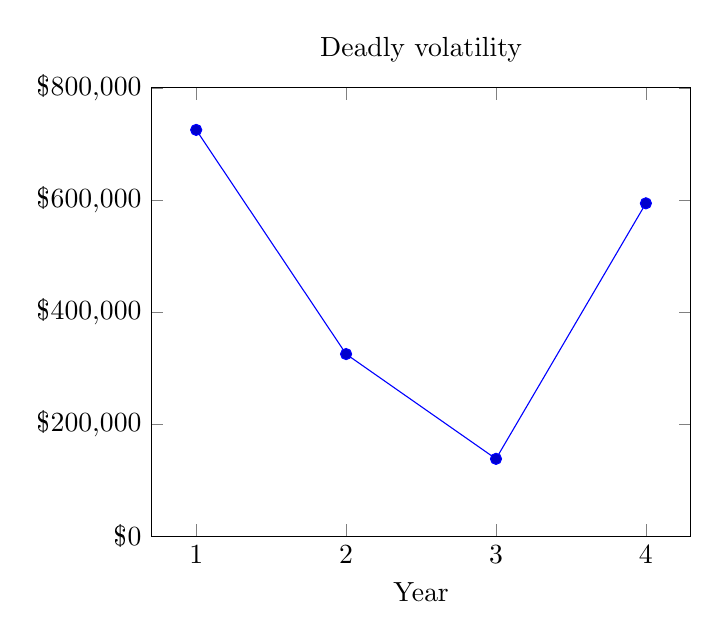
\begin{tikzpicture}
    \begin{axis}[
      xlabel=Year,
      xtick=data,
      title=Deadly volatility,
      yticklabel={\$$\pgfmathprintnumber{\tick}$},
      yticklabel style={/pgf/number format/fixed},
      scaled ticks=false,
      ymin=0,
      ymax=800000,
    ]
    \addplot coordinates {
      (1, 725000)
      (2, 325000)
      (3, 138000)
      (4, 594000)
    };
    \end{axis}
  \end{tikzpicture}
\end{figure}

Of course, this example exhibits major volatility, but it demonstrates the point. The more volatility, the more you will spend down shares of your portfolio during lean years, so the less volatility, the better you will preserve your portfolio in those years.

Notice too, in this example, that the drop happened in the first years. It could just as easily have been the reverse, which would have the opposite effect. If you entered into major bull market in the first few years, you'd need to spend much fewer shares in order to withdraw your \$30,000, thereby increasing your portfolio value. Then, if the same drop happens ten years later, your portfolio would have been much stronger to withstand the same onslaught. So, it all depends on timing and volatility. I have found volatility risk to be one of the greatest investment risks you face when you start taking withdrawals. If you lose a huge portion of your portfolio right off the bat like that, and yet you still need to withdraw money, then your financial future will be in peril.

That's exactly what happened to me. I retired in February, 2008. The stock market immediately started dropping, and then in October, I faced the greatest stock market crash since The Great Depression. There was a high positive correlation between all of the components in my portfolio, so even diversification didn't save me. I ended up losing 25\% of my money. I had some contingency plans, but this was beyond what I could reasonably plan for, so my resolve was tested, yet again.

I dropped everything I was doing for six months, and focused entirely on the catastrophe. I panicked a few times, then focused, then panicked some more, and focused again. It was scary. First, I looked for even more ways to cut costs in ways that didn't significantly harm my quality of life. Then I pulled out the contingency plans. I purposely had several ``nice-to-have'' expenses that I could easily cut in case of emergency. I cut them all, and I was still drowning. I started cutting out some ``\emph{really}-nice-to-have'' expenses. Then I started looking for a cheaper place to live.

Meanwhile, I was researching investing again, scouring websites, reading books, trying to figure out how I could have better prevented this disaster, and how I can better avoid it in the future. Most importantly, I was trying to figure out how to stop the bleeding immediately. The conclusion I reached is that there was nowhere to hide. The drop was across the board. Then I did something very naughty: I sold everything.

\emph{Don't try this at home.} If your portfolio is evaporating before your eyes, selling is usually the worst thing you could possibly do. It's the nature of volatility that your investments will recover, and it's the nature of our psychology that your fear will keep you from buying back in before that happens.

My choice to sell wasn't so much out of panic. It was a decision I made after a lot of thought and research. It was a big risk, and I knew that. I sold for two reasons. The first reason is that it became clear to me that it was only the beginning. The second, and more important reason, is that it also became clear that this was a unique recession, one never before seen in history. All investment wisdom is based on what we've learned from history. There was no precedent for this. Extreme times called for extreme measures. I may have an investment ``religion,'' but I'm not a fundamentalist. I can still believe in buying and holding index funds, but that doesn't mean that I'm unwilling to make exceptions at the right times, like when I see my entire retirement dream vanishing before my eyes. In the worst case, I'd have to go back to work and start over again, but at least I would go down fighting.

I researched for another couple of weeks, and then started buying back in, slowly at first, with a whole new portfolio. This new portfolio has several features that I will describe next. I designed it to not only withstand future catastrophes better, but to also take advantage of the current low prices and therefore bring me out even further ahead than when the whole mess started.

The choices I made turned out to be excellent, overall. I was right that it was only the beginning. It was beneficial to sell when I did and buy back in at lower prices, even though I didn't time it perfectly (no one can). I'd promised myself that I would buy back in \emph{before} it felt safe, so as to avert the risk of not being there for the big recovery. But I did take a huge risk. What if it recovered quickly? I'd have sold at the lowest point, losing a huge opportunity for recovery.

\section{Investing for growth or income}
As I researched for my new portfolio, I was considering the one disadvantage I had as a retiree: I was taking out regular withdrawals. If this weren't the case, I could have easily ridden out the storm and watched everything recover completely. But I knew even a year or two of severe losses would be much more severe for me long-term if I took withdrawals in those years. Before I retired, I hadn't thought much about this problem, but I had planned to re-think things once I retired and had some more time on my hands. I just didn't expect to need it so soon.

Portfolios tend to be classified as either \emph{income, growth,} or some combination of both. An income portfolio is one that is designed to give pay-outs at regular intervals, with very little volatility. A growth portfolio is one that is designed to grow over time, with major volatility. This captures the big trade-off of investing—risk is always rewarded with greater growth over time.

I also considered the other unique aspect of my situation: my retirement was at a young age. That means that I will be holding these investments longer than most retirees, so I have longer to ride out the volatility, even though I will be taking withdrawals along the way. What I needed was a portfolio that was less volatile than pure growth portfolios, more volatile than pure income portfolios, but still provided steady income along the way. What I needed was a combination growth and income portfolio.

As I researched this, one thing that became clear was that I needed more dividends. Dividends are regular payments made to shareholders, from the income the companies earn. Dividends do tend to go down during recessions, but not as significantly as the share prices. If I could invest in things that gave more dividends, I realized, if I could take a larger portion of my withdrawals from those dividends, then I wouldn't need to sell so many shares during recessions. I'd avoided dividends before because they're taxed at a higher rate than long term capital gains, but I'm in a much lower tax bracket now that I'm retired, so avoiding dividends for tax purposes isn't a big deal. I'll talk more about taxes at the end of the chapter.

I read a great book, called \emph{A Random Walk Down Wall Street,} that showed how difficult it is to predict the market, and how mutual funds that do great in one year often do lousy in the years that follow. It talks about what statistical randomness looks like, and showed that it's in the nature of randomness to sometimes not look random. The reason for this is in our own psychology. We tend to see patterns where none exist. So, these mutual funds that seem to perform well are in fact just exhibiting statistically random behavior. They advertise their past performances which, just as in the case of a series of coin tosses, say nothing about their future results.

Another thing I learned, or rather, rediscovered, is costs. I read another book called \emph{Common Sense on Mutual Funds.} I hadn't before seen such a thorough treatment on the effects of fees, and this book explained why. Fees are like the dirty little secret of the mutual fund and brokerage industries. It's in the interest of these industries to avoid talking about them. The only reason they talk about fees to the extent they do is because the Securities Exchange Commission forces them to, and I realized after reading this book that they still don't tell the half of it.

When you put this together with the Random Walk theory, you can see how fees significantly effect returns. If these funds are essentially random, and past performance of the funds have little or no bearing on future results, then the only predictable way to maximize future results is to minimize costs. You've seen in Chapter 2 how small costs at regular intervals add up astonishingly quickly, especially when that money could have been invested. That's exactly the situation we have here.

The best way to invest, then, is to minimize the fees by minimizing the management. Since the fund managers can't do any better than just invest randomly, you don't need fund managers to be quite so active, which means you can pay them less. This also results in the managers making fewer trades (called \emph{turnover}) which also incurs less taxes for the shareholders.

Index funds, like any other mutual funds, are purchased from the mutual fund company itself, each share representing underlying stocks and bonds owned by the fund company. If \emph{you} buy or sell many shares, \emph{they} must buy or sell many shares. This incurs significant costs to the shareholders, so responsible fund companies will institute limits and penalties on how often shareholders may buy and sell their shares. Another issue with mutual funds, particularly troublesome in volatile times, is that they have up to a one day delay in their share price, or \emph{NAV.} At the end of each day, they update the NAV, and when you buy, you pay the NAV on the next cycle, so you don't know what that NAV will be. That can be risky.

Something else I discovered during this time is \emph{Exchange-Traded Funds,} or \emph{ETFs.} These are a lot like index funds, but they're traded like stocks. You buy them from a stock broker just as you would stocks. There are no limits or penalties on buying or selling shares, since the brokers deal with such large volumes of them, called \emph{creation units.} Since the fund company doesn't have to buy or sell frequently, they tend to be more tax-efficient as well. And since ETFs are handled by stock brokers, rather than the fund companies that offer them, they also have lower trading, management, and marketing costs than even most index funds.

ETFs were initially used by day traders, but their low costs, tax efficiency, and lower volatility risk also made them great candidates for buying and holding. In fact, buying and holding ETFs minimizes their only disadvantage, which is the trading fees. Brokers charge brokerage fees to trade them, just as they do for stocks. If you use ETFs, I recommend you use a discount brokerage firm. Also, only buy ETFs that have a low \emph{average bid/ask spread.} This is the difference between the amount you pay to buy a share and the amount you could sell it for at any given time. It's a hidden cost of trading that must be accounted for. Most ETF companies should be able to tell you the average bid/ask spread of their ETFs.

As I said, I may have an investment religion, but I'm not a fundamentalist. My ``religion'' is buying and holding a diverse allocation of broad index funds. This is almost always the strategy I use. However, sometimes I use a small portion of my portfolio to speculate with more targeted investments. This actually serves my asset allocation in a way, because the goal in Modern Portfolio Theory is to have many different investments that behave differently, and individual stocks and sectors sometimes behave differently than the market as a whole.

The key to trading, more so than with buying and holding, is to buy low and sell high. This sounds simple but it's not easy. For one thing, what does ``low'' mean? Valuing stocks, ETFs, and mutual funds isn't as straightforward as it looks. For most things we buy, we can compare the price we pay to see which one is cheaper. So it makes sense that we'd be able to compare the share prices of the investments we want to buy. Even some articles in the media do this, which betrays their ignorance of the stock market. A stock price is fairly arbitrary. A company can change it whenever they want, by ``splitting,'' which means they offer twice as many shares at half the price. This makes it look ``cheap'' which is a big reason they do it, but it's worth exactly the same as it was before, because there are now twice as many available.

For example, if you had a giant candy bar, and you broke it up into 20 pieces and sold them for \$1 each, then the candy bar is worth \$20. But if you broke it up into 40 pieces and sold them for \$0.50 each, then the candy bar is still worth \$20. Buying two half-pieces for \$0.50 each is the same as buying one whole piece for \$1. You need to do the same thing for the investments you buy. Multiply the share price by the shares outstanding. This is called the \emph{market capitalization} or \emph{market cap} and you can usually look it up in the key statistics for the investment.

However, just because an investment has a low market cap still doesn't mean that it's a bargain. Usually, a company will have a low market cap for a good reason. Maybe they don't earn much money, or their future is in doubt. So you need to look at other data to decide whether it's a good deal. One such number is the \emph{Price/Earnings ratio,} or \emph{P/E ratio,} which is the stock price divided by the annual earnings, or how much each dollar of annual earnings costs you. This will be lower for investments that have poor future prospects or is not expected to grow much, and higher for investments that are expected to grow. Like any business you buy, you'd pay more for one that is expected to grow quickly.

Another number is the \emph{Price/Book ratio,} which is the stock price divided by the assets owned by the company, or how much each dollar of assets costs you. Another number is the \emph{Price/Sales ratio,} which is the stock price divided by the annual sales, or how much each dollar of annual sales costs you. Sales are different from earnings, in that they don't account for the expenses a company has. For example, if a company has a low Price/Sales ratio but a high Price/Earnings ratio, it means that the company is actually really good at earning money, but they're also really good at spending it. Just as you saw in Chapters 1 and 2, both the income and spending components are important. It's often easier to cut costs than it is to get more income, so if you believe the company will do a good job at cutting costs, then this might be a good deal.

After you look at all these numbers, you'll know whether the price is low, but you still won't know why. Like, if you're shopping for a shirt, and you see the price is \$5, you'll know the price is low, but you won't know why. It might be because the shirt is damaged. It's up to you as a buyer to examine the shirt, and ask the clerk questions about it, to make sure it's the bargain you hope it is. Likewise, you need to examine an investment, read their news, read message boards where investors discuss it, and maybe call their investor relations hotline, to determine if it's a bargain.

But the hardest part of buying low and selling high is our psychology. Our impulse is to do the opposite. When things are going well, we want more of it. When things are bad, we want out before it gets worse. So, it's essential that you be a contrarian. You need to be on a shopping spree when everyone else is talking about apocalypse. You need to be a cynic and start selling off when everyone is talking about how great things are and that it can only get better.

When there's a stock market crash, panic ensues. People sell off their investments out of fear. Their fear overpowers their rationality, so they'll sell at any price, even if that price is obviously lower than the company is worth. During the 2008 crash, some of America's strongest companies were trading at lower than their book value (Price/Book was less than 1). That means that these sellers were saying, in essence, that these companies had no hope of ever turning a profit. They were saying that these companies weren't even worth the property they owned! They were in such a panic to sell that they're practically giving these companies away. This is an excellent time to snap up some great deals. I bought some shares of a few companies during this time. One of them tripled and another doubled in value in less than a year before I sold it.

I'd be a wealthy man if I'd put my entire portfolio in these companies, but that's very risky. People tried that with Enron, what they thought was a ``can't-lose'' company, and they lost their entire life savings. The reason for diversity is that you don't know which companies will succeed. It's a random walk. During a severe recession, even some of America's strongest companies can be in dire straights. It is actually possible they'd burn up all their cash before going out of business, so it's not like the fears are completely unfounded. But it doesn't hurt to devote a small portion of your portfolio to such speculation, if you believe in the company.

I also do this with ``sectors'' I believe in, or that are known to be good investments for both growth and income. A sector is a portion of the stock market that meets a certain criteria, usually an industry. For example, I have a telecommunications ETFs, because they have decent growth while offering huge dividends.

Something else I did was over-invest in stock funds. By the time I bought back in, I had quite a bit more stock exposure than I did before. This caused a bit more volatility during that year as the market struggled to incorporate all the news, but it didn't last very long. First it started to stabilize, then I saw a nice recovery, and a year later, I sold some of them off and bought back into bonds. This allowed me to take advantage of the under-priced stocks. I do this whenever I re-balance. I over-compensate, either buying more bonds or more stocks than are in my target allocation, to take advantage of the market extremes.

One good way to determine this is with the \emph{P/E10 ratio.} The P/E10 ratio is a measurement of the prices of the stock market as a whole compared to its earnings over 10 years. Over the long run, the prices tend to track earnings. This ratio has averaged out to about 20. If it varies from this significantly, it's usually a good sign that things are under-valued or over-valued.

\section{Designing your portfolio}
So, what should your portfolio look like? There are many ways to answer that question. Investing is a personal thing, and depends on a lot of factors specific to you: your age, values, goals, fears, and hopes. So I can't tell you what your portfolio should look like, but I can explain the process I used to come up with my portfolio.

First, I sought out great minds that I trusted. One of these, Warren Buffett, doesn't write much, and the books about him talk about his method, which isn't quite so relevant for the average investor. But there were five others that have written good books: Bernard Malkiel, John C. Bogle, William Bernstein, Richard A. Ferri, and Roger Gibson. They each made their own portfolio recommendations. I adjusted each of them for roughly my target allocation of stocks and bonds. Then I compared them side-by-side. They didn't always overlap, so I sometimes had to fill in the blanks with guesses.  I've included these five portfolios at the end of this section.

I looked at this table of model portfolios and came up with an amount for each investment that made the most sense for me, from what I'd read and from my own experience. For the most part, the portfolio I came up with is an amalgamation of all five portfolios, with my own personal twist. For example, some of my portfolio is for speculation, as I explained earlier. I also substituted \emph{mid-cap} (middle-sized companies) for \emph{large-cap} (large companies), because there are several companies in every large-cap fund that I despise, particularly Microsoft and Apple. Mid-cap funds tend behave very much like large-cap funds anyway, so that made sense for me.

First, divide your allocation between stocks and bonds. This depends on your age and risk tolerance. The more bonds you have in your portfolio, the less volatile it will be, but also the less it will grow. The younger you are, the longer you have to ride out the storms, so you'll want more stocks, because that will give you more growth. If you're older, you'll want more bonds because you don't have the same luxury of time to ride out the volatility. Likewise for risk tolerance: if you tend to freak out when there are crashes, you'll want more bonds, but if you know you can keep your cool, you'll want more stocks so you can take advantage of their superior growth. Additionally, once you start taking withdrawals, no matter how old you are, you'll want more bonds, because you're much more susceptible to volatility.


Start with an allocation based on your age. Here's a good rule-of-thumb: If you're under 40, your allocation should be 90\% stocks, 10\% bonds. Starting at age 40, add 3 percentage points of bonds every 2 years. For example, at 40, change your allocation to 87\%/13\%, at 42, change it to 84\%/16\%, etc.

Now adjust for your risk tolerance. If you tend to freak out a little during recessions, add 10 percentage points of bonds. If you tend to freak out a lot, add 10 more. This is your portfolio, so it's completely your choice how much adjustment you need to make for you to feel comfortable. If you choose something too aggressive for your risk aversion, and you end up selling out of fear, then that extra little bit of growth you got would do you no good, so if you're not sure, be conservative and lean toward more bonds rather than less.

Once you start taking withdrawals, add another 5 percentage points of bonds, and also consider investing more in dividend-bearing investments.

Next, you must decide how much exposure you want to international markets. International investing has historically been important for diversification because they offer relatively low correlations with domestic investments, although that has been changing as our economy becomes more global. Some argue that it's pointless to invest internationally, because it's just more risk with little benefit. Others argue that international is the way to go because they believe America will no longer be the economic super power it once was. Most experts believe it's best to have at least some exposure to international.

You should now have two divisions of your portfolio, or four asset classes. For example, if you decided on 60/40 for your stock/bond mix and 80/20 for your domestic/international mix, your portfolio would be 48\% domestic stocks, 12\% international stocks, 32\% domestic bonds, and 8\% international bonds. Now it's time to explain all the many ways you can divide up each of these four asset classes.

For stocks, you have a few different ways you can diversify. One is company size. Large companies perform differently than small companies, so you'll want to have some of both. There are four main size categories: large-cap, mid-cap, small-cap, and micro-cap. Another way to diversify stocks is \emph{growth} versus \emph{value,} which I explained in the Investment Basics section. Both perform roughly just as well, but they tend to behave a little differently, which makes them good candidates for diversification, so you should have some of both. You could get them as separate funds, or you could get them both in a \emph{blend fund.}

In international stocks, you have similar distinctions as above, but you can also diversify by region. The main geographical categories are Europe, Pacific Rim, and Emerging Markets. Pacific Rim includes many non-European, first world countries like Japan, Singapore, and Australia. Emerging Markets includes many of the third world countries. Of the three, Europe is known to behave the most like American stocks and is the least risky and volatile. Emerging Markets behaves the least like American stocks and is the most risky and volatile. Pacific Rim is in the middle, both in correlation and risk. You should probably own some of all three, either separately or together in one fund.

There are non-company stocks you can also buy for good diversification effect. One is the \emph{REIT,} which stands for \emph{Real Estate Investment Trust.} Rather than owning parts of a company, you own parts of corporate real estate. You're paid rent in the form of dividends. You can also buy precious metals and other commodities. Gold is known to be extremely volatile and doesn't perform well long-term, but it may be good to have some in your mix because it tends to have a very low correlation with most other stocks, and is also a tool for lowering inflation risk.

For bonds, you can diversify based on type, quality, and term. There are government bonds and corporate bonds. Some government bonds worth looking into are \emph{TIPS} and \emph{GNMA.} TIPS is designed to protect you against inflation, which is a good way to lower inflation risk. GNMA is the government mortgage bonds.

The two main categories of quality are \emph{investment grade} and \emph{high yield.} Investment grade bonds are bonds issued by entities with a good credit rating and a history of not defaulting. High yield used to be called \emph{junk bonds} but that turned out to be bad marketing. They refer to entities with poor credit ratings and some history of defaulting, but their rates are much higher to compensate for that risk. So, you can expect the risk and volatility of high yield bonds to be greater than investment grade bonds, but you can also expect higher long-term growth.

There are short-term, intermediate-term, and long-term bonds. This refers to how long until the loans need to be paid back. The longer the term, the higher the risk, but also the higher the rates. However, long-term bonds don't tend to give enough growth to compensate for its greater risk, so it's better to just stick to short-term and intermediate-term bonds.

International bonds aren't easy to find. As far as I know, there's only one company, DFA, that offers international bond funds that distinguishes between the above three factors, and that company doesn't actually offer these funds to the general public. The amount of international bonds you'll own will probably not be very high anyway, so this doesn't matter much, and you can just buy a generic international bond fund. However, there are some good international bond ETFs available to the general public.

How much you divide your portfolio between each of these many types of investments doesn't matter as much as the main two divisions between stocks/bonds and domestic/international. Different experts have different opinions on this, but there do tend to be a few common patterns: Growth and value are often divided equally, and it's common to have more large-cap and mid-cap than small-cap and micro-cap, more domestic than international, more Pacific Rim and Europe than Emerging Markets, and more short-term and intermediate-term investment-grade bonds than high yield bonds, TIPS, and GNMA.

As an example of a complete asset allocation, the following page is a table with my own portfolio, next to the five model portfolios I based it on, from the books \emph{Asset Allocation, All About Asset Allocation, A Random Walk Down Wall Street, Common Sense on Mutual Funds,} and \emph{The Intelligent Asset Allocator.} Some of these books didn't spell it out exactly like it is on this table, but I needed some way to compare them side-by-side, so I made some guesses in some cases.

\begin{table}[ht]
\caption{Model portfolios}
\centering
\begin{tabular}{l l r r r r r r}
\\\hline
\\\hline
& \textbf{Symbol} & \textbf{Mason} & \textbf{Gibson} & \textbf{Ferri} & \textbf{Malkiel} & \textbf{Bogle} & \textbf{Bernstein}\\
\hline
\textbf{\emph{Stocks}} & & \textbf{\emph{69.50\%}} & \textbf{\emph{65.00\%}} & \textbf{\emph{60.00\%}} & \textbf{\emph{65.00\%}} & \textbf{\emph{60.00\%}} & \textbf{\emph{60.00\%}}\\
\textbf{U.S. Equity} & & \textbf{54.50\%} & \textbf{46.00\%} & \textbf{48.00\%} & \textbf{47.00\%} & \textbf{54.00\%} & \textbf{46.80\%}\\
Large growth & VIG & 0.00\% & 7.50\% & 15.00\% & 11.50\% & 15.00\% & 6.00\%\\
Large value & VYM, VIG, VOX & 24.00\% & 7.50\% & 15.00\% & 11.50\% & 15.00\% & 21.00\%\\
Mid-cap growth & VOT & 4.00\% & 0.00\% & 0.00\% & 0.00\% & 3.00\% & 0.00\%\\
Mid-cap value & & 0.00\% & 0.00\% & 0.00\% & 0.00\% & 3.00\% & 0.00\%\\
Small growth & VBK & 3.00\% & 6.50\% & 0.00\% & 7.00\% & 6.00\% & 1.50\%\\
Small value & VBR & 9.00\% & 6.50\% & 9.60\% & 7.00\% & 6.00\% & 10.50\%\\
Microcap & VTWO & 2.50\% & 0.00\% & 2.40\% & 0.00\% & 0.00\% & 0.00\%\\
Real estate & VNQ & 6.00\% & 12.00\% & 6.00\% & 10.00\% & 0.00\% & 6.00\%\\
Speculation & Varies & 5.00\% & 0.00\% & 0.00\% & 0.00\% & 0.00\% & 0.00\%\\
Gold & IAU & 1.00\% & 6.00\% & 0.00\% & 0.00\% & 0.00\% & 1.80\%\\
Oil \& Gas & & 0.00\% & 0.00\% & 0.00\% & 0.00\% & 6.00\% & 0.00\%\\
\textbf{Intl. Equity} & & \textbf{15.00\%} & \textbf{19.00\%} & \textbf{12.00\%} & \textbf{18.00\%} & \textbf{6.00\%} & \textbf{13.20\%}\\
Pacific Rim large & VPL & 4.00\% & 5.00\% & 3.60\% & 6.00\% & 2.00\% & 3.00\%\\
Europe large & VGK & 4.00\% & 5.00\% & 3.60\% & 6.00\% & 2.00\% & 3.00\%\\
Intl. small cap & SCZ & 2.50\% & 5.00\% & 2.40\% & 0.00\% & 0.00\% & 0.00\%\\
Intl. value & IDV & 2.00\% & 0.00\% & 0.00\% & 0.00\% & 0.00\% & 4.20\%\\
Emerging markets & VWO & 2.50\% & 4.00\% & 2.40\% & 6.00\% & 2.00\% & 3.00\%\\
\textbf{\emph{Fixed income}} & & \textbf{\emph{30.50\%}} & \textbf{\emph{35.00\%}} & \textbf{\emph{40.00\%}} & \textbf{\emph{35.00\%}} & \textbf{\emph{30.00\%}}\\
\textbf{Bonds} & & \textbf{25.50\%} & \textbf{30.00\%} & \textbf{38.00\%} & \textbf{30.00\%} & \textbf{35.00\%} & \textbf{30.00\%}\\
Invest. grade & BND & 6.00\% & 9.00\% & 7.92\% & 12.50\% & 35.00\% & 10.00\%\\
High-yield & VWEHX & 2.50\% & 3.00\% & 7.92\% & 0.00\% & 0.00\% & 0.00\%\\
TIPS & SCHP & 3.50\% & 0.00\% & 7.92\% & 5.00\% & 0.00\% & 10.00\%\\
GNMA & VMBS & 4.00\% & 0.00\% & 0.00\% & 12.50\% & 0.00\% & 0.00\%\\
Short-term & BSV & 8.00\% & 10.00\% & 10.29\% & 0.00\% 0.00\% 10.00\%\\
Intl. bonds & PCY & 1.50\% & 8.00\% & 3.96\% & 0.00\% & 0.00\% & 0.00\%\\
\textbf{Cash} & & \textbf{5.00\%} & \textbf{5.00\%} & \textbf{2.00\%} & \textbf{5.00\%} & \textbf{5.00\%} & \textbf{10.00\%}\\
Money market & & 5.00\% & 5.00\% & 2.00\% & 5.00\% & 5.00\% & 10.00\%\\
\hline
\end{tabular}
\end{table}

As you can see, there's quite a bit of difference of opinion between the experts, and that's not even accounting for individual preferences, needs, age, goals, and risk aversion. This is really something you need to customize. I made many choices that disagreed with the experts because I weighed the arguments made in the various books and decided where I stood on those, and whether they applied to me. I favor value and mid-cap companies. I want dividends. I add a small speculative element. I don't want to invest in oil or gas. And then I tweaked the numbers based on my age, goal, and risk tolerance. I also occasionally tweak this target allocation as things change or as I incorporate new information.

Not only is creating a target asset allocation the most personal part of investing, it's also the most important to get right. Most investing experts agree that your asset allocation has far more impact on the performance and risk of your investments than which funds you choose. So, don't spend all your time shopping for funds. Spend more time refining your target allocation. There are many good books on this subject, several of which are included in the resources. Do your homework and get this right.

\section{Taxes}
One logistical concern that every good investor should be aware of is taxes. Many people are painfully aware of how much payroll taxes they pay, so it's ironic that so few account for them in their investments. This is probably because investment taxes are relatively invisible compared to payroll taxes. They don't show up on their paychecks or monthly statements. But like every recurring, incidental expense, taxes some of those expenses that can make a huge difference over time. Taxes are just as important as fees. In a sense, they \emph{are} fees, just paid to a different payee.

Taxes are very political. Taxes are how we pay for government services, and the major division between each political philosophy is how this money is collected and spent. Pretty much everyone disagrees with at least something the government spends money on, and doesn't want to support that with their life energy. On the other hand, we all use the services the government provides. Many resent it, while many others are grateful for those services and are glad to support them.

That's exactly the problem with taxes. They support everything, the good, the bad, and the ugly. We're not allowed to opt out of taxes. That's a good thing, because if they could, citizens could unfairly pick and choose what to pay for, but still be free to benefit from them. We can't afford to run a government on the honor system. Many services can't reasonably or efficiently be deregulated and parceled out to commercial entities. Some things are inherently a commons. Enforcing air quality, for example. Either everyone has clean air or no one does. There's no way to choose to pay to get clean air or choose to opt out. This is a basic economic truth that some political perspectives ignore or gloss over.

Taxes should be fair, and it's up to our elected officials to create a fair tax system. They will offer credits, deductions, and adjustments to incentivize certain things and allow for exceptions to the basic tax rules. Your job as an investor is to learn about which of these are relevant for you and take advantage of them. In other words, your goal is to minimize the taxes you're required to pay.

Unfortunately, the tax system is not fair. It's designed predominantly to benefit the rich, which the Occupy Wall Street started making people aware of in the early 2010's. Even though the IRS tables are based on a graduated tax system, designed to require those who earn the most to pay the most in taxes, there are tons of adjustments, credits, and deductions that were designed for the rich that often outweighs anything extra they pay. As you begin saving more money, you'll notice that you become eligible for more tax advantages.

The most fundamental aspect of our tax system is that it is based on earning money and spending money. Income tax is for the money you earn, and sales tax is for the money you spend. Financial independence involves minimizing the amount of money you spend in order to minimize the money you earn. Therefore, by the very nature of the tax system, the closer you get to financial independence, the less you'll be required to pay in taxes. You'll be spending less, so you'll be paying less sales tax. Your food and drug costs will be a larger portion of your total spending, which are not taxed at all. You'll be earning less, so you'll pay less in income taxes, at a lower tax bracket. More of your income will come from investments, which is taxed at a lower rate than salary.

Interest and dividends are taxed at your normal tax rate. Then there's capital gains. These are the gains you get from selling an investment at a higher price than you paid for it. The IRS distinguishes between two holding periods: short-term capital gains are gains you made on investments that you held for one year or less. These are also taxed at your normal tax rate. However, long-term capital gains for investments you held for more than one year are taxed at very low rates. If your tax bracket is 25\% or higher, you only pay only 15\% for your long term capital gains, which is nearly half of what you'd normally pay. If your tax bracket is 10\% or 15\%, you pay zero taxes on your long-term capital gains!

Hopefully, your tax strategy can involve keeping your income as low as possible, so you can pay zero taxes on your long-term capital gains. Take a look at your current tax schedule to see what income this means for you. You will also want to minimize your short-term capital gains. That means only selling your investments if you've held them for at least a year. If you re-balance your portfolio no more frequently than one year and one day, then this should be taken care of for you.

You should also minimize interest and dividends, since these are taxed at your normal rates. This is especially true while you're earning a lot and saving for financial independence, since you'll be in a higher tax bracket. There are a few ways to minimize dividends. One is to invest inside of a tax shelter, which I will talk about shortly. Another is \emph{tax-managed funds.} Another is to focus on growth funds more than value funds. Once you go into a lower tax bracket, however, it's not quite as important to minimize dividends. I have found that the added advantage of a more stable income outweighs the need to minimize dividends for tax purposes once I achieved financial independence and started taking regular withdrawals.

You should also minimize the \emph{turnover} in any funds outside of tax shelters. Turnover is the percentage of the holdings in a fund that are bought and sold each year. You're not only taxed on the capital gains that you get from buying and selling the fund as a whole, but also all from the buying and selling that happens \emph{within the fund} throughout the year. These taxes can really add up fast for high-turnover funds. Look for funds with less than a 50\% annual turnover. Index funds are, by definition, extremely low-turnover funds. If you're looking for funds to invest in, look for such low-turnover funds. Otherwise, put these investments in a tax shelter or look for tax-managed funds.

\emph{Tax shelters} protect your investments from taxes, mainly for retirement purposes. One tax shelter is the 401(k) and 403(b) retirement plans (named after the section of the tax code that created them). You get these through an employer. They deduct a certain amount from your paychecks. Many of them also \emph{match} your contributions, which means that they will pay some amount to your retirement plan for each amount you pay. You will not be taxed on this or its growth until you retire. There are limits to this, and my recommendation is that you take advantage of this as much as you can, up to the limit. Once you leave your job, you may \emph{roll over} (which is just a fancy way of saying ``moving'') your money from your 401(k) or 403(b) plans into an IRA or Roth IRA.

An \emph{Individual Retirement Account,} also called a \emph{IRA} or \emph{traditional IRA,} does not depend on your job. IRAs provide the same benefits as an employer-sponsored plan with far more flexibility, but with lower contribution limits. Unlike an employer-sponsored plan, you can invest your IRA in anything you want--stocks, bonds, savings accounts, CDs, pretty much anything. The IRA itself is just a tax mechanism. Whichever investment vehicle you choose, the IRA only means that you don't have to pay taxes on what you contribute to it or on its growth until it comes time to withdraw it.

For the 401(k), 403(b), and IRA, you will be taxed when you take withdrawals. This is called \emph{tax deferral.} This is very much to your advantage because your earnings will have grown tax-free for all those years, and you will probably be in a lower tax bracket when you start taking withdrawals.

In an IRA, you're not taxed on what goes in, but on what comes out. A Roth IRA is kind of the opposite in this sense. You're taxed on what goes in, but not on what comes out. Otherwise, it's very similar to a traditional IRA. Whether you would be better off contributing to an IRA or Roth IRA depends on your tax bracket. If you're in a high tax bracket, you'd be better off contributing to an IRA, because you won't be taxed until you're in a lower tax bracket later. You can also later convert an IRA to a Roth IRA and get taxed right away if you go into a lower tax bracket.

Roth IRAs are usually more advantageous than IRAs. As long as you're not in a high tax bracket, it's better to pay taxes right away and not pay any taxes on its growth, because over time, the growth of investments tends to far overshadow the original contributions. Another advantage of the Roth IRA is that you can withdraw the original contributions any time you want. The one exception is that you must wait 5 years before doing so for any money you've converted from a traditional IRA to a Roth IRA.

Another tax shelter is a \emph{Health Savings Account} or \emph{HSA.} There are health insurance plans that provide these. You put money into this account tax-free, which can grow over time. Then when you get sick, you can the withdraw money tax-free. This is an excellent option for people who are relatively healthy, due to their extremely low monthly premiums and tax savings. There are also tax shelters for saving for education, but most tax shelters are designed for retirement.

The government has a very specific idea of what retirement means. On the surface, their definitions may seem to differ from those who want financial independence in the form of early retirement. The standard rule is that you can't retire until you're $59 \frac{1}{2}$ years old. However, they provide a little known exception to this rule for early retirees: you may withdraw your money from your IRA or Roth IRA at regular intervals, on a schedule according to your life expectancy. This is called the \emph{72(t) exception.} All the IRS cares about is that you're actually retired, and not just taking money out whenever you feel like it. Therefore, once you start taking withdrawals on a schedule, you must continue doing so indefinitely.

This might not be necessary, however. If you're saving quickly, you will hit your tax shelter contribution limits, and you will need to save money outside of your tax shelter. Once you start taking withdrawals, start with money outside of your tax shelter, and once you've depleted that, then start taking regular withdrawals from your IRA or Roth IRA. Once you've started taking withdrawals from a Roth IRA, you will be able to withdraw all your original contributions tax-free, and will only need to use the 72(t) schedule once you've depleted that.

I actually pay \emph{zero taxes,} legally and with no loopholes. First, I invested heavily in my 401(k), paying zero taxes going in. Once I became financially independent, I rolled over everything into an IRA. Since I retired so early, I have plenty of time to slowly convert my money from my IRA to a Roth IRA. Selling everything and buying back in with a whole new portfolio means I reported huge losses that will take me years to recapture. Deductions or losses from previous years eliminate the taxes on the small conversions from my IRA to Roth IRA each year. Then once it's all in my Roth IRA, I can withdraw all of my money tax-free. My expenses are so low that, after deductions, my income is 10\% or 15\% tax bracket, which means that all long-term capital gains from anything not in the IRA or Roth IRA will also be tax-free. Of course, this takes a fair amount of careful tax planning, but it's completely legal and safe.

As you can see, the government loves people who have enough money to invest. Another type of rich person the government loves is the homeowner. Many of the biggest costs for homeowners are actually deductible from taxes. Mortgage interest and property taxes are entirely tax deductible. The greatest tax benefit of owning a home is that any gains you get from selling it for more than you bought it are also completely tax-free. You get even more benefit if you rent out some rooms in your home, because this allows you to deduct a large portion of your maintenence and repair expenses as well.

In summary, the best way to minimize the tax you're required to pay is to earn and spend as little as possible, use tax shelters, own and live in a rental home, use tax-managed funds outside of your tax shelters, and keep high dividend and high turnover funds in your tax shelters. Maximize your contributions to your 401(k) or 403(b) first, then maximize your contributions to your IRA or Roth IRA, and then invest normally. IRA is tax-free going in and taxed coming out, while Roth IRA is taxed going in and tax-free coming out. It's better to use a Roth IRA if you're in a lower tax bracket. It's possible to pay zero taxes if you keep your income low enough and you slowly convert your IRA to a Roth IRA over time, with enough deductions or capital losses to capture those conversions.

\newpage
\section{Resources}
\begin{itemize}
\item \textbf{\emph{A Random Walk Down Wall Street,} by Burton Malkiel.} This is the best investing book I've ever read. I consider it essential reading. It explains everything you need to know about investing, in the most down-to-earth fashion I've ever seen, but without dumbing it down. It demonstrates the Random Walk theory of investing. It is a little long-winded, but it's worth it.
\item \textbf{\emph{Common Sense on Mutual Funds} by John C. Bogle.} If you can only read one investing book, read A Random Walk, but if you can read two, read Common Sense. When you read this book, you'll understand just how absolutely vital it is to minimize investment costs. Although this book is a little dry at times, the way Bogle exposes the evils of the Mutual Fund industry gave me a ferver of almost religious proportions, which explains why many in the index fund industry call him a saint.

\item \textbf{\emph{All About Asset Allocation} by Richard A. Ferri.} If you can only read two investing books, read A Random Walk and Common Sense, but if you can read three, read All About Asset Allocation. Other books explain how investing works, but fall short when it comes to the nuts-and-bolts of putting together an actual portfolio. This book assumes you know how investing works, and just explains how asset allocation works and how to put together a good portfolio.

\item \textbf{\url{http://www.vanguard.com/}} -- The only investment company I completely trust.

\item \textbf{\url{https://personal.vanguard.com/us/whatweoffer/advice}} -- Vanguard's offerings of the three options described in the Investing made easy section: hiring a financial planner, one-time financial planning, and balanced funds.

\item \textbf{\url{http://www.multpl.com/}} -- This is a simple chart that shows where the P/E10 ratio has been, and where it is currently. It also provides simples charts for several other economic indicators. 
\end{itemize}
